\documentclass[12pt, a4paper]{book}

\usepackage[T1]{fontenc}
\usepackage[utf8]{inputenc}
\usepackage[charter, cal=cmcal]{mathdesign}
\usepackage[scaled=0.92]{helvet}
\usepackage{geometry}
\geometry{a4paper, top=30mm, bottom=30mm, inner=32mm, outer=25mm, marginparwidth=18mm}

\usepackage{amsmath, amsthm}
\usepackage[version=4]{mhchem}
\usepackage{graphicx}
\usepackage[dvipsnames,svgnames,table]{xcolor}
\usepackage{tikz}
\usetikzlibrary{arrows.meta, shapes.geometric, positioning,
                calc, backgrounds, patterns}
\usepackage{pgfplots}
\pgfplotsset{compat=1.18}
\usepackage{tcolorbox}
\tcbuselibrary{skins, breakable, theorems}
\usepackage{titlesec}
\usepackage{fancyhdr}
\usepackage{enumitem}
\usepackage{booktabs}
\usepackage{array}
\usepackage{multicol}
\usepackage{caption}
\usepackage{parskip}
\usepackage{siunitx}
\usepackage{pifont}
\usepackage[colorlinks=true, linkcolor=BrickRed,
            urlcolor=NavyBlue, citecolor=ForestGreen]{hyperref}

% ── Colours ───────────────────────────────────────────────────────────────────
\definecolor{JourneyColor}{HTML}{4A235A}
\definecolor{ModuleColor}{HTML}{6C3483}
\definecolor{PuzzleColor}{HTML}{1A5276}
\definecolor{DiscoveryColor}{HTML}{B7950B}
\definecolor{WarningColor}{HTML}{C0392B}
\definecolor{ProblemColor}{HTML}{117A65}
\definecolor{ReflectColor}{HTML}{1D6A39}
\definecolor{HistoryColor}{HTML}{6E2F1A}
\definecolor{ElectronBlue}{HTML}{1565C0}
\definecolor{NucleusRed}{HTML}{B71C1C}
\definecolor{SpinUp}{HTML}{1A5276}
\definecolor{SpinDown}{HTML}{922B21}

% ── Boxes ─────────────────────────────────────────────────────────────────────
\newtcolorbox{puzzlebox}[1][]{enhanced,breakable,
  colback=PuzzleColor!6,colframe=PuzzleColor,fonttitle=\bfseries\sffamily,
  title={The Puzzle},attach boxed title to top left={yshift=-2mm,xshift=6mm},
  boxed title style={colback=PuzzleColor},borderline west={3pt}{0pt}{PuzzleColor},#1}

\newtcolorbox{discoverybox}[1][]{enhanced,breakable,
  colback=DiscoveryColor!8,colframe=DiscoveryColor,fonttitle=\bfseries\sffamily,
  title={Discovery},attach boxed title to top left={yshift=-2mm,xshift=6mm},
  boxed title style={colback=DiscoveryColor},borderline west={3pt}{0pt}{DiscoveryColor},#1}

\newtcolorbox{problembox}[1][]{enhanced,breakable,
  colback=ProblemColor!5,colframe=ProblemColor,fonttitle=\bfseries\sffamily,
  title={Problems},attach boxed title to top left={yshift=-2mm,xshift=6mm},
  boxed title style={colback=ProblemColor},borderline west={3pt}{0pt}{ProblemColor},#1}

\newtcolorbox{deepbox}[1][]{enhanced,breakable,
  colback=JourneyColor!5,colframe=JourneyColor,fonttitle=\bfseries\sffamily,
  title={Deep Problems},attach boxed title to top left={yshift=-2mm,xshift=6mm},
  boxed title style={colback=JourneyColor},borderline west={4pt}{0pt}{JourneyColor},#1}

\newtcolorbox{historybox}[1][]{enhanced,breakable,
  colback=HistoryColor!7,colframe=HistoryColor!60,fonttitle=\bfseries\sffamily\small,
  title={Historical Note},attach boxed title to top left={yshift=-2mm,xshift=6mm},
  boxed title style={colback=HistoryColor!80},#1}

\newtcolorbox{reflectionbox}[1][]{enhanced,breakable,
  colback=ReflectColor!6,colframe=ReflectColor,fonttitle=\bfseries\sffamily,
  title={Reflection},attach boxed title to top left={yshift=-2mm,xshift=6mm},
  boxed title style={colback=ReflectColor},borderline west={3pt}{0pt}{ReflectColor},#1}

\newtcolorbox{modelbreaks}[1][]{enhanced,breakable,
  colback=WarningColor!6,colframe=WarningColor,fonttitle=\bfseries\sffamily,
  title={Where This Model Breaks},attach boxed title to top left={yshift=-2mm,xshift=6mm},
  boxed title style={colback=WarningColor},borderline west={4pt}{0pt}{WarningColor},#1}

\newtcolorbox{namedconcept}[2][]{enhanced,
  colback=ModuleColor!6,colframe=ModuleColor,fonttitle=\bfseries\sffamily\large,
  title={#2},attach boxed title to top left={yshift=-2mm,xshift=6mm},
  boxed title style={colback=ModuleColor},#1}

\newtcolorbox{synthbox}[1][]{enhanced,breakable,
  colback=JourneyColor!8,colframe=JourneyColor!70,fonttitle=\bfseries\sffamily,
  title={Journey 2 Synthesis},attach boxed title to top left={yshift=-2mm,xshift=6mm},
  boxed title style={colback=JourneyColor!70},borderline west={4pt}{0pt}{JourneyColor},#1}

% ── Section formatting ────────────────────────────────────────────────────────
\titleformat{\chapter}[display]
  {\normalfont\sffamily\huge\bfseries\color{JourneyColor}}
  {\textcolor{JourneyColor!60}{\chaptertitlename\ \thechapter}}{10pt}{\Huge}
  [\vspace{2pt}\textcolor{JourneyColor}{\titlerule[1.5pt]}]
\titleformat{\section}
  {\normalfont\sffamily\Large\bfseries\color{ModuleColor}}
  {\thesection}{1em}{}[\textcolor{ModuleColor!40}{\titlerule[0.6pt]}]
\titleformat{\subsection}
  {\normalfont\sffamily\large\bfseries\color{JourneyColor!80}}{\thesubsection}{1em}{}
\titleformat{\subsubsection}
  {\normalfont\sffamily\normalsize\bfseries}{\thesubsubsection}{1em}{}

\pagestyle{fancy}
\fancyhf{}
\fancyhead[LE]{\small\sffamily\textcolor{JourneyColor}{\leftmark}}
\fancyhead[RO]{\small\sffamily\textcolor{ModuleColor}{\rightmark}}
\fancyfoot[C]{\small\thepage}
\renewcommand{\headrulewidth}{0.4pt}

\newcommand{\newterm}[1]{\textit{\textcolor{DiscoveryColor}{#1}}}
\newcommand{\important}[1]{\textcolor{ModuleColor}{\textbf{#1}}}

% ── Helper for electron box diagrams ──────────────────────────────────────────
\newcommand{\ebox}[1]{%
  \begin{tikzpicture}[baseline=-1pt, scale=0.9]
    \draw[thick, JourneyColor!60] (0,0) rectangle (0.55,0.55);
    \ifnum#1=1
      \draw[-{Stealth[length=4pt]}, thick, SpinUp] (0.275,0.1) -- (0.275,0.45);
    \fi
    \ifnum#1=2
      \draw[-{Stealth[length=4pt]}, thick, SpinUp] (0.2,0.1) -- (0.2,0.45);
      \draw[-{Stealth[length=4pt]}, thick, SpinDown] (0.35,0.45) -- (0.35,0.1);
    \fi
  \end{tikzpicture}%
}
\newcommand{\emptybox}{%
  
\begin{tikzpicture}[baseline=-1pt, scale=0.9]
    \draw[thick, JourneyColor!30] (0,0) rectangle (0.55,0.55);
  \end{tikzpicture}%
}

% ══════════════════════════════════════════════════════════════════════════════
\begin{document}
\setcounter{chapter}{1}
\chapter[Journey 2 --- Architecture of the Atom]
        {Journey Two\\[8pt]
         \textcolor{ModuleColor}{\large Architecture of the Atom}}
\setcounter{section}{6}

% ══════════════════════════════════════════════════════════════════════════════
\section{Module 2.7 --- Orbitals, Quantum Numbers, and Electron Configuration}
\label{sec:mod2.7}

\subsection*{Motivation}

Hydrogen is the simplest atom --- one proton, one electron.
Its wave functions can be solved exactly.
But chemistry is built from heavier atoms: carbon (6 electrons),
nitrogen (7), oxygen (8), iron (26), uranium (92).

How do we describe multi-electron atoms?
How do we decide which electrons go into which orbitals?
Why do atoms have the periodic properties they do?

The answers rest on two principles that have nothing to do
with the Schr\"{o}dinger equation itself: the
\newterm{Pauli exclusion principle} and \newterm{Hund's rules}.
Together with the orbital structure of the hydrogen solutions,
they explain the structure of the entire periodic table.

This module completes Journey~2 by building the quantum
mechanical foundation that Journey~3 will use to read
the periodic table as a map of electron structure.

% ─── Section: The Four Quantum Numbers ───────────────────────────────────────
\subsection{The Four Quantum Numbers}

The Schr\"{o}dinger equation for hydrogen produces wave
functions labelled by three quantum numbers.
A fourth --- electron spin --- is required to explain
all experimental observations.

\begin{namedconcept}{The Four Quantum Numbers}
\begin{center}
\begin{tabular}{lllp{6cm}}
\toprule
Symbol & Name & Allowed values & Physical meaning \\
\midrule
$n$ & Principal & $1, 2, 3, \ldots$ & Energy shell; average distance from nucleus \\[4pt]
$\ell$ & Angular momentum & $0, 1, \ldots, n-1$ & Shape of the orbital; orbital angular momentum $= \sqrt{\ell(\ell+1)}\,\hbar$ \\[4pt]
$m_\ell$ & Magnetic & $-\ell, \ldots, 0, \ldots, +\ell$ & Orientation of the orbital; $z$-component of angular momentum $= m_\ell\hbar$ \\[4pt]
$m_s$ & Spin & $+\tfrac{1}{2}$ or $-\tfrac{1}{2}$ & Intrinsic angular momentum of the electron \\
\bottomrule
\end{tabular}
\end{center}

The letter labels for $\ell$: $\ell=0$ is $s$, $\ell=1$ is $p$,
$\ell=2$ is $d$, $\ell=3$ is $f$
(from spectroscopic terms: \textbf{s}harp, \textbf{p}rincipal,
\textbf{d}iffuse, \textbf{f}undamental).
\end{namedconcept}

\vspace{0.5em}

The number of orbitals with a given $n$ and $\ell$
is $2\ell+1$ (the number of allowed $m_\ell$ values).
Including both spin states, each orbital holds 2 electrons.

\begin{center}
\begin{tabular}{cclcc}
\toprule
$n$ & $\ell$ & Subshell & Orbitals ($2\ell+1$) & Max electrons \\
\midrule
1 & 0 & $1s$ & 1 & 2 \\
2 & 0 & $2s$ & 1 & 2 \\
2 & 1 & $2p$ & 3 & 6 \\
3 & 0 & $3s$ & 1 & 2 \\
3 & 1 & $3p$ & 3 & 6 \\
3 & 2 & $3d$ & 5 & 10 \\
4 & 0 & $4s$ & 1 & 2 \\
4 & 1 & $4p$ & 3 & 6 \\
4 & 2 & $4d$ & 5 & 10 \\
4 & 3 & $4f$ & 7 & 14 \\
\bottomrule
\end{tabular}
\end{center}

\begin{puzzlebox}
\begin{enumerate}[label=(\alph*), leftmargin=*]
  \item Count the total electrons that fit in shell $n=1$,
        $n=2$, $n=3$, $n=4$.
        These are $2, 8, 18, 32$.
        Do you recognise these numbers?
        Where do they appear in the periodic table?

  \item For $n=4$, list all valid combinations of
        $(n, \ell, m_\ell, m_s)$.
        How many are there?
        Show this equals $2n^2 = 32$.

  \item The quantum number $\ell$ determines the
        \emph{shape} of the orbital.
        $\ell = 0$: spherical. $\ell = 1$: dumb-bell.
        $\ell = 2$: cloverleaf (or doughnut).
        Why might the shape of an electron's orbital
        matter for chemistry?
        (Hint: consider how atoms bond to each other.)

  \item In hydrogen, all orbitals with the same $n$
        have the same energy (degenerate).
        In multi-electron atoms, the $2s$ orbital
        has lower energy than $2p$.
        Why? (Think about which orbital has more probability
        density near the nucleus, where the nucleus's
        attraction is strongest.)
\end{enumerate}
\end{puzzlebox}

% ─── Section: Electron Spin ───────────────────────────────────────────────────
\subsection{Electron Spin: An Intrinsic Property}

In 1922, Otto Stern and Walther Gerlach sent silver atoms
through an inhomogeneous magnetic field.
Classical physics predicted the beam would spread into
a continuous band.
Instead, the beam split into exactly two.

The electron has an intrinsic \newterm{spin} angular momentum
that can point in only two directions relative to any axis:
``up'' ($m_s = +\tfrac{1}{2}$) or ``down'' ($m_s = -\tfrac{1}{2}$).

\begin{center}
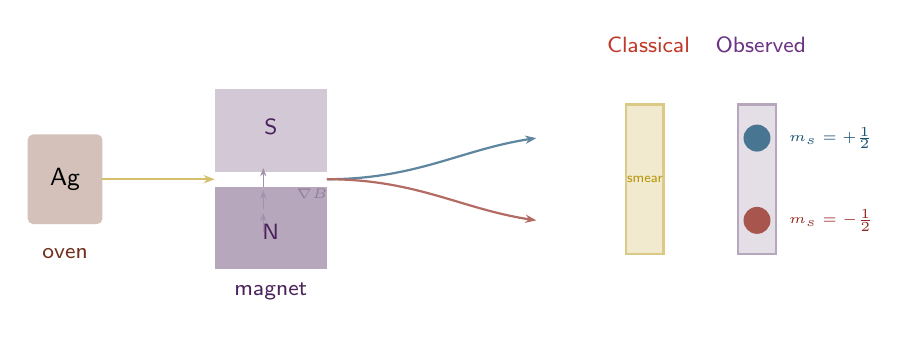
\begin{tikzpicture}[every node/.style={font=\sffamily\small}, scale=0.95]
  % Oven
  \fill[HistoryColor!30, rounded corners=2pt]
    (-7.0,-0.6) rectangle (-6.0,0.6);
  \node at (-6.5,0) {Ag};
  \node[font=\sffamily\footnotesize, text=HistoryColor] at (-6.5,-1.0) {oven};

  % Beam
  \draw[thick, DiscoveryColor!60, -{Stealth[length=4pt]}]
    (-6.0,0) -- (-4.5,0);

  % Magnet poles
  \fill[JourneyColor!40] (-4.5,-1.2) -- (-4.5,-0.1) -- (-3.0,-0.1)
    -- (-3.0,-1.2) -- cycle;
  \fill[JourneyColor!25] (-4.5, 0.1) -- (-4.5, 1.2) -- (-3.0, 1.2)
    -- (-3.0, 0.1) -- cycle;
  \node[font=\sffamily\footnotesize, text=JourneyColor] at (-3.75,-0.7) {N};
  \node[font=\sffamily\footnotesize, text=JourneyColor] at (-3.75, 0.7) {S};
  \node[font=\sffamily\footnotesize, text=JourneyColor] at (-3.75,-1.5) {magnet};

  % Field gradient arrows
  \foreach \y in {-0.7,-0.4,-0.1} {
    \draw[-{Stealth[length=3pt]}, thin, JourneyColor!50]
      (-3.85,\y) -- (-3.85, \y+0.25);
  }
  \node[font=\sffamily\tiny, text=JourneyColor!60] at (-3.2,-0.2) {$\nabla B$};

  % Classical prediction: continuous smear
  \begin{scope}[xshift=1.5cm]
    \node[font=\sffamily\footnotesize, text=WarningColor] at (-0.2, 1.8) {Classical};
    \fill[DiscoveryColor!20] (-0.5,-1.0) rectangle (0,1.0);
    \draw[DiscoveryColor!50, thick] (-0.5,-1.0) rectangle (0,1.0);
    \node[font=\sffamily\tiny, text=DiscoveryColor] at (-0.25,0) {smear};
  \end{scope}

  % Quantum result: two spots
  \begin{scope}[xshift=3.0cm]
    \node[font=\sffamily\footnotesize, text=ModuleColor] at (-0.2, 1.8) {Observed};
    \fill[JourneyColor!15] (-0.5,-1.0) rectangle (0,1.0);
    \draw[JourneyColor!40, thick] (-0.5,-1.0) rectangle (0,1.0);
    \fill[SpinUp!80]   (-0.25, 0.55) circle (0.18cm);
    \fill[SpinDown!80] (-0.25,-0.55) circle (0.18cm);
    \node[font=\sffamily\tiny, text=SpinUp,   right] at (0.05, 0.55) {$m_s=+\tfrac{1}{2}$};
    \node[font=\sffamily\tiny, text=SpinDown, right] at (0.05,-0.55) {$m_s=-\tfrac{1}{2}$};
  \end{scope}

  % Split beam
  \draw[thick, SpinUp!70, -{Stealth[length=4pt]}]
    (-3.0,0) .. controls (-1.8,0) and (-1.2,0.4) .. (-0.2,0.55);
  \draw[thick, SpinDown!70, -{Stealth[length=4pt]}]
    (-3.0,0) .. controls (-1.8,0) and (-1.2,-0.4) .. (-0.2,-0.55);

\end{tikzpicture}
\end{center}

\vspace{0.5em}

Spin is a purely quantum property --- there is no classical
analogue.
It is not the electron physically spinning (an electron
has no measurable spatial extent to spin).
It is an intrinsic angular momentum with magnitude
$\frac{\sqrt{3}}{2}\hbar$ and no classical explanation.

% ─── Section: Pauli Exclusion Principle ──────────────────────────────────────
\subsection{The Pauli Exclusion Principle}

In 1925, Wolfgang Pauli proposed the principle that explains
why electrons fill shells in the pattern they do:

\begin{namedconcept}{Pauli Exclusion Principle (1925)}
No two electrons in the same atom can have the same
set of four quantum numbers $(n, \ell, m_\ell, m_s)$.

Equivalently: each orbital (defined by $n$, $\ell$, $m_\ell$)
can hold at most \textbf{two electrons}, and they must have
opposite spins.
\end{namedconcept}

\vspace{0.5em}

This principle is not derived from the Schr\"{o}dinger equation.
It is an additional postulate, required to explain
the structure of multi-electron atoms.
Its deep justification lies in the quantum statistics
of identical particles (the spin-statistics theorem),
which is beyond our scope here.

The practical consequence: electrons fill available orbitals
starting from the lowest energy, with at most two per orbital.
This is the \newterm{Aufbau principle} (German: ``building up'').

% ─── Section: Energy Ordering of Orbitals ────────────────────────────────────
\subsection{Energy Ordering and the Aufbau Principle}

In multi-electron atoms, the $2s$ orbital is lower in energy
than $2p$, because $s$ orbitals have higher electron
density near the nucleus (``penetration'').
The $3d$ orbital is actually higher in energy than $4s$
for neutral atoms, leading to the famous crossing in the
fourth row.

The energy ordering (approximately) is:
\[
  1s < 2s < 2p < 3s < 3p < 4s < 3d < 4p < 5s < 4d < 5p < \cdots
\]

\begin{center}
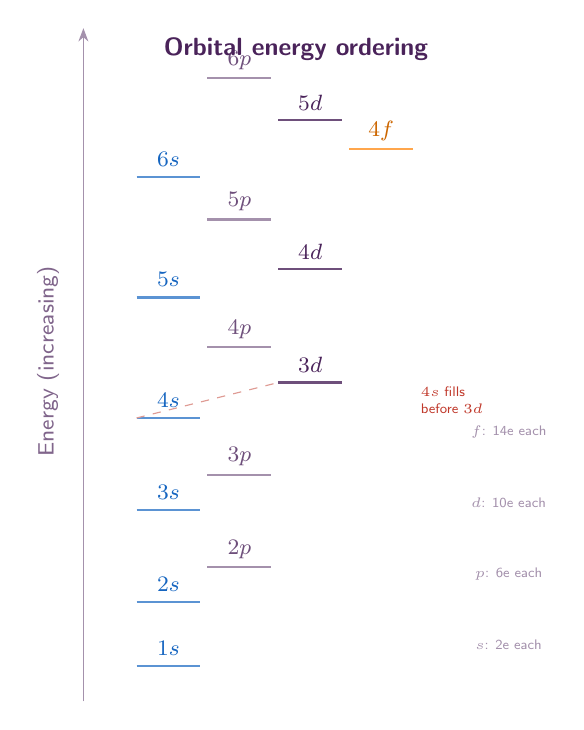
\begin{tikzpicture}[every node/.style={font=\sffamily\small}, scale=0.9]
  % Energy axis
  \draw[-{Stealth}, thin, JourneyColor!50] (0,0) -- (0,9.5);
  \node[rotate=90, font=\sffamily\footnotesize, text=JourneyColor!70]
    at (-0.5, 4.8) {Energy (increasing)};

  % Draw orbital levels with labels
  % Format: xpos, ypos, label, color
  % s orbitals (blue)
  \foreach \xp/\yp/\lbl in {
    1.2/0.5/{$1s$}, 1.2/1.4/{$2s$}, 1.2/2.7/{$3s$},
    1.2/4.0/{$4s$}, 1.2/5.7/{$5s$}, 1.2/7.4/{$6s$}
  }{
    \draw[thick, ElectronBlue!70] (\xp-0.45,\yp) -- (\xp+0.45,\yp);
    \node[font=\sffamily\footnotesize, text=ElectronBlue] at (\xp,\yp+0.25) {\lbl};
  }
  % p orbitals (purple)
  \foreach \xp/\yp/\lbl in {
    2.2/1.9/{$2p$}, 2.2/3.2/{$3p$},
    2.2/5.0/{$4p$}, 2.2/6.8/{$5p$}, 2.2/8.8/{$6p$}
  }{
    \draw[thick, JourneyColor!50] (\xp-0.45,\yp) -- (\xp+0.45,\yp);
    \node[font=\sffamily\footnotesize, text=JourneyColor!80] at (\xp,\yp+0.25) {\lbl};
  }
  % d orbitals (dark)
  \foreach \xp/\yp/\lbl in {
    3.2/4.5/{$3d$}, 3.2/6.1/{$4d$}, 3.2/8.2/{$5d$}
  }{
    \draw[thick, JourneyColor!80] (\xp-0.45,\yp) -- (\xp+0.45,\yp);
    \node[font=\sffamily\footnotesize, text=JourneyColor] at (\xp,\yp+0.25) {\lbl};
  }
  % f orbital (amber)
  \draw[thick, orange!70] (4.2-0.45,7.8) -- (4.2+0.45,7.8);
  \node[font=\sffamily\footnotesize, text=orange!80!black] at (4.2,8.05) {$4f$};

  % Capacity annotations on right
  \node[font=\sffamily\tiny, text=JourneyColor!50] at (6.0, 0.8) {$s$: 2e each};
  \node[font=\sffamily\tiny, text=JourneyColor!50] at (6.0, 1.8) {$p$: 6e each};
  \node[font=\sffamily\tiny, text=JourneyColor!50] at (6.0, 2.8) {$d$: 10e each};
  \node[font=\sffamily\tiny, text=JourneyColor!50] at (6.0, 3.8) {$f$: 14e each};

  % Key crossing: 4s below 3d annotation
  \draw[dashed, thin, WarningColor!50] (0.75,4.0) -- (2.75,4.5);
  \node[font=\sffamily\tiny, text=WarningColor, align=left]
    at (5.2, 4.25) {$4s$ fills\\before $3d$};

  % Title
  \node[font=\sffamily\small\bfseries, color=JourneyColor]
    at (3.0, 9.2) {Orbital energy ordering};

\end{tikzpicture}
\end{center}

% ─── Section: Writing Electron Configurations ─────────────────────────────────
\subsection{Writing Electron Configurations}

The \newterm{electron configuration} of an atom lists
how electrons are distributed among orbitals.

\begin{center}
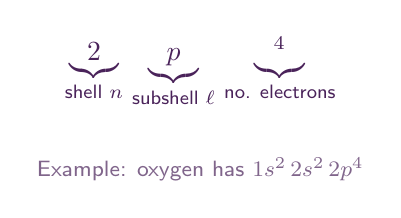
\begin{tikzpicture}[every node/.style={font=\sffamily\small}, scale=0.95]
  % Notation explanation
  \node[font=\sffamily\normalsize, color=JourneyColor]
    at (3.0, 1.0) {$\underbrace{2}_{\text{shell }n}\,
                    \underbrace{p}_{\text{subshell }\ell}\,
                    \underbrace{^4}_{\text{no. electrons}}$};
  \node[font=\sffamily\footnotesize, color=JourneyColor!70]
    at (3.0, -0.3) {Example: oxygen has $1s^2\,2s^2\,2p^4$};
\end{tikzpicture}
\end{center}

\vspace{0.3em}

\begin{center}
\begin{tabular}{lllll}
\toprule
$Z$ & Element & Config & Orbital diagram & Group \\
\midrule
1  & H  & $1s^1$                 & \ebox{1}                    & 1 \\
2  & He & $1s^2$                 & \ebox{2}                    & 18 \\
3  & Li & $[He]\,2s^1$           & \ebox{2}\,\ebox{1}          & 1 \\
4  & Be & $[He]\,2s^2$           & \ebox{2}\,\ebox{2}          & 2 \\
5  & B  & $[He]\,2s^2\,2p^1$    & \ebox{2}\,\ebox{2}\,\ebox{1}\,\emptybox\,\emptybox & 13 \\
6  & C  & $[He]\,2s^2\,2p^2$    & \ebox{2}\,\ebox{2}\,\ebox{1}\,\ebox{1}\,\emptybox  & 14 \\
7  & N  & $[He]\,2s^2\,2p^3$    & \ebox{2}\,\ebox{2}\,\ebox{1}\,\ebox{1}\,\ebox{1}   & 15 \\
8  & O  & $[He]\,2s^2\,2p^4$    & \ebox{2}\,\ebox{2}\,\ebox{2}\,\ebox{1}\,\ebox{1}   & 16 \\
9  & F  & $[He]\,2s^2\,2p^5$    & \ebox{2}\,\ebox{2}\,\ebox{2}\,\ebox{2}\,\ebox{1}   & 17 \\
10 & Ne & $[He]\,2s^2\,2p^6$    & \ebox{2}\,\ebox{2}\,\ebox{2}\,\ebox{2}\,\ebox{2}   & 18 \\
\midrule
11 & Na & $[Ne]\,3s^1$           & \ebox{2}\,\ebox{1}          & 1 \\
18 & Ar & $[Ne]\,3s^2\,3p^6$    & (full $n=3$)                & 18 \\
19 & K  & $[Ar]\,4s^1$           & \ebox{1}                    & 1 \\
20 & Ca & $[Ar]\,4s^2$           & \ebox{2}                    & 2 \\
26 & Fe & $[Ar]\,3d^6\,4s^2$    & (6 in $3d$, 2 in $4s$)     & 8 \\
\bottomrule
\end{tabular}
\end{center}

Notice the pattern: Li and Na both have a single electron
in an $s$ orbital beyond a full shell --- Group 1 (alkali metals).
Ne and Ar both end with a full $p$ subshell --- Group 18 (noble gases).

\important{The periodic table is a map of electron configurations.}

% ─── Section: Hund's Rules ────────────────────────────────────────────────────
\subsection{Hund's Rules: Filling Degenerate Orbitals}

When electrons fill a subshell with multiple degenerate orbitals
(same energy), they do not pair up immediately.
Instead they spread out, one per orbital, with parallel spins.

\begin{namedconcept}{Hund's First Rule}
When filling degenerate orbitals, electrons occupy separate
orbitals with \textbf{parallel spins} before any orbital is
doubly occupied.
This minimises electron-electron repulsion and (by the
spin correlation of quantum mechanics) stabilises the
configuration.
\end{namedconcept}

\vspace{0.5em}

This explains the orbital diagrams for carbon, nitrogen,
and oxygen in the table above.
Carbon's two $2p$ electrons go into separate orbitals,
not the same one:
\begin{center}
  \ebox{2}\hspace{6pt}\ebox{2}\hspace{6pt}
  \ebox{1}\hspace{2pt}\ebox{1}\hspace{2pt}\emptybox\hspace{10pt}
  (carbon, correct: Hund's rule obeyed)

  \vspace{4pt}

  \ebox{2}\hspace{6pt}\ebox{2}\hspace{6pt}
  \ebox{2}\hspace{2pt}\emptybox\hspace{2pt}\emptybox\hspace{10pt}
  (carbon, incorrect: Hund's rule violated)
\end{center}

\begin{problembox}
\begin{enumerate}[label=\textbf{\arabic*.}]
  \item Write the full electron configurations for:
        \begin{enumerate}[label=(\alph*)]
          \item \ce{Na} ($Z=11$)
          \item \ce{Cl} ($Z=17$)
          \item \ce{Ca} ($Z=20$)
          \item \ce{Fe} ($Z=26$)
          \item \ce{Br} ($Z=35$)
          \item \ce{Kr} ($Z=36$)
        \end{enumerate}

  \item Using orbital box diagrams, show the electron
        configuration of the $3d$ subshell for:
        \begin{enumerate}[label=(\alph*)]
          \item \ce{Sc} ($Z=21$): $[Ar]\,3d^1\,4s^2$
          \item \ce{V} ($Z=23$): $[Ar]\,3d^3\,4s^2$
          \item \ce{Mn} ($Z=25$): $[Ar]\,3d^5\,4s^2$
          \item \ce{Fe} ($Z=26$): $[Ar]\,3d^6\,4s^2$
          \item \ce{Zn} ($Z=30$): $[Ar]\,3d^{10}\,4s^2$
        \end{enumerate}
        For each, state whether the atom has unpaired electrons
        and hence whether it is magnetic (paramagnetic).

  \item Chromium ($Z=24$) and copper ($Z=29$) have anomalous
        configurations:
        \ce{Cr}: $[Ar]\,3d^5\,4s^1$ (not $3d^4\,4s^2$)
        \ce{Cu}: $[Ar]\,3d^{10}\,4s^1$ (not $3d^9\,4s^2$)
        \begin{enumerate}[label=(\alph*)]
          \item Explain these anomalies using the
                extra stability of half-filled ($d^5$)
                and fully filled ($d^{10}$) subshells.
          \item How many unpaired electrons does \ce{Cr} have?
          \item Is \ce{Cu} paramagnetic in its ground state?
        \end{enumerate}
\end{enumerate}
\end{problembox}

% ─── Section: Periodic Properties from Configuration ─────────────────────────
\subsection{Periodic Properties Explained by Configuration}

The electron configuration directly explains several
periodic trends --- quantities that vary predictably
across the periodic table.

\subsubsection{Atomic Radius}

Atomic radius generally \emph{decreases} across a period
(left to right) and \emph{increases} down a group.

\begin{itemize}[nosep, leftmargin=2em]
  \item Across a period: $Z$ increases, $n$ stays constant.
        More protons pull the same shell inward.
  \item Down a group: a new shell is added.
        Outer electrons are further from the nucleus.
\end{itemize}

\subsubsection{Ionisation Energy}

\newterm{Ionisation energy} (IE) is the energy to remove
the outermost electron.
It generally increases across a period and decreases down a group.

\begin{center}
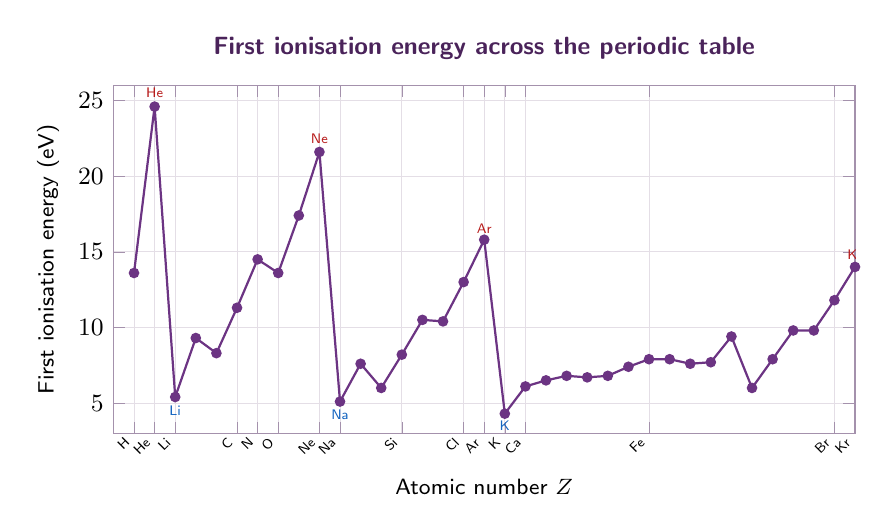
\begin{tikzpicture}[every node/.style={font=\sffamily\small}]
  \begin{axis}[
    width=11cm, height=6cm,
    xlabel={Atomic number $Z$},
    ylabel={First ionisation energy (eV)},
    xmin=0, xmax=36,
    ymin=3, ymax=26,
    xtick={1,2,3,6,7,8,10,11,14,17,18,19,20,26,35,36},
    xticklabels={H,He,Li,C,N,O,Ne,Na,Si,Cl,Ar,K,Ca,Fe,Br,Kr},
    x tick label style={font=\sffamily\tiny, rotate=45, anchor=east},
    ytick={5,10,15,20,25},
    grid=both,
    grid style={line width=0.3pt, draw=JourneyColor!15},
    axis line style={color=JourneyColor!50},
    tick style={color=JourneyColor!50},
    title style={font=\sffamily\small\bfseries, color=JourneyColor},
    title={First ionisation energy across the periodic table},
    label style={font=\sffamily\footnotesize}
  ]
    \addplot[thick, color=ModuleColor, mark=*, mark size=1.5pt]
      coordinates {
        (1,13.6)(2,24.6)(3,5.4)(4,9.3)(5,8.3)(6,11.3)(7,14.5)
        (8,13.6)(9,17.4)(10,21.6)(11,5.1)(12,7.6)(13,6.0)(14,8.2)
        (15,10.5)(16,10.4)(17,13.0)(18,15.8)(19,4.3)(20,6.1)
        (21,6.5)(22,6.8)(23,6.7)(24,6.8)(25,7.4)(26,7.9)(27,7.9)
        (28,7.6)(29,7.7)(30,9.4)(31,6.0)(32,7.9)(33,9.8)(34,9.8)
        (35,11.8)(36,14.0)
      };

    % Annotate noble gases
    \node[font=\sffamily\tiny, text=NucleusRed] at (axis cs:2,25.5) {He};
    \node[font=\sffamily\tiny, text=NucleusRed] at (axis cs:10,22.5) {Ne};
    \node[font=\sffamily\tiny, text=NucleusRed] at (axis cs:18,16.5) {Ar};
    \node[font=\sffamily\tiny, text=NucleusRed] at (axis cs:36,14.8) {Kr};

    % Annotate alkali metals
    \node[font=\sffamily\tiny, text=ElectronBlue] at (axis cs:3,4.5) {Li};
    \node[font=\sffamily\tiny, text=ElectronBlue] at (axis cs:11,4.2) {Na};
    \node[font=\sffamily\tiny, text=ElectronBlue] at (axis cs:19,3.5) {K};
  \end{axis}
\end{tikzpicture}
\end{center}

\vspace{0.3em}

The pattern is striking:
\begin{itemize}[nosep, leftmargin=2em]
  \item Noble gases (He, Ne, Ar, Kr) have the highest IE ---
        full subshells, very stable.
  \item Alkali metals (Li, Na, K) have the lowest IE ---
        one electron beyond a full shell, easy to remove.
  \item Nitrogen has slightly higher IE than oxygen
        (half-filled $2p^3$ is extra-stable by Hund's rule).
\end{itemize}

\subsubsection{Electronegativity and Chemical Reactivity}

Elements on the upper right (F, O, N, Cl) are highly
\newterm{electronegative} --- they strongly attract electrons
in bonds.
This is because they need only one or two more electrons
to complete their valence shell, and their high $Z$ pulls
electrons in strongly.

Elements on the lower left (Cs, Ba, Fr, Ra) are the most reactive
metals --- their valence electrons are far from the nucleus,
weakly held, and easily donated to electronegative partners.

\emph{This is chemistry arising directly from electron configuration.}

% ─── Section: Journey 2 Synthesis ────────────────────────────────────────────
\subsection*{Journey 2 Synthesis: The Architecture of the Atom}

\begin{synthbox}
Journey 2 began with a single question: what are atoms made of?
It ends with a complete, quantum mechanical picture.

\medskip
\begin{center}
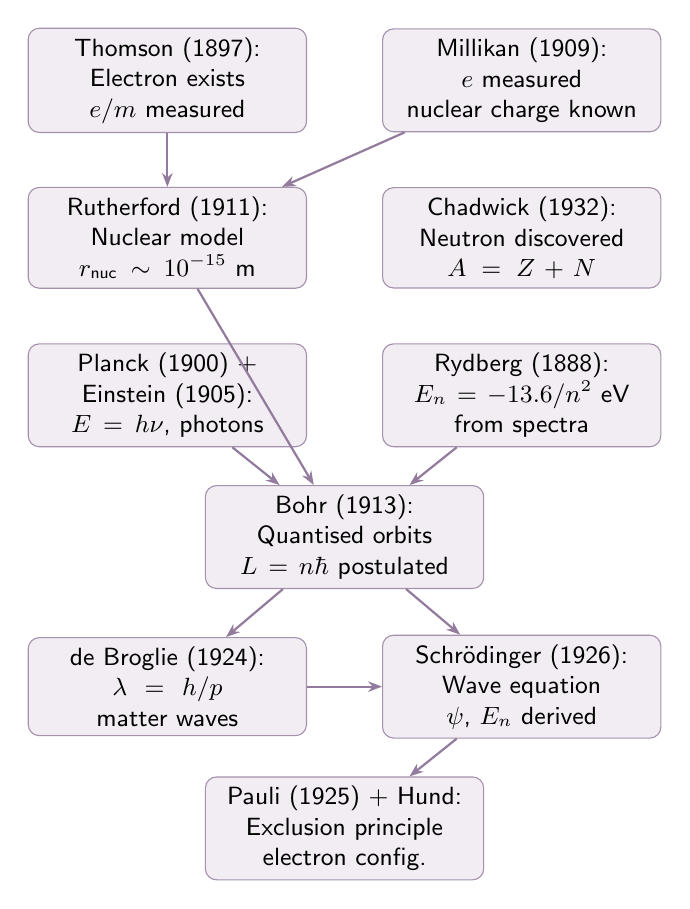
\begin{tikzpicture}[
  every node/.style={font=\sffamily\small, align=center},
  box/.style={draw=JourneyColor!50, fill=JourneyColor!8, rounded corners=4pt,
              minimum width=3.5cm, minimum height=1.0cm, text width=3.3cm},
  arr/.style={-{Stealth[length=5pt]}, thick, JourneyColor!60}
]
  \node[box] (thom) at (0, 8.0) {Thomson (1897):\\Electron exists\\$e/m$ measured};
  \node[box] (mill) at (4.5, 8.0) {Millikan (1909):\\$e$ measured\\nuclear charge known};
  \node[box] (ruth) at (0, 6.0) {Rutherford (1911):\\Nuclear model\\$r_\text{nuc} \sim 10^{-15}$ m};
  \node[box] (chad) at (4.5, 6.0) {Chadwick (1932):\\Neutron discovered\\$A = Z+N$};
  \node[box] (plan) at (0, 4.0) {Planck (1900) +\\Einstein (1905):\\$E = h\nu$, photons};
  \node[box] (spec) at (4.5, 4.0) {Rydberg (1888):\\$E_n = -13.6/n^2$ eV\\from spectra};
  \node[box] (bohr) at (2.25, 2.2) {Bohr (1913):\\Quantised orbits\\$L = n\hbar$ postulated};
  \node[box] (debr) at (0, 0.3) {de Broglie (1924):\\$\lambda = h/p$\\matter waves};
  \node[box] (schr) at (4.5, 0.3) {Schr\"{o}dinger (1926):\\Wave equation\\$\psi$, $E_n$ derived};
  \node[box] (paul) at (2.25,-1.5) {Pauli (1925) + Hund:\\Exclusion principle\\electron config.};

  \draw[arr] (thom) -- (ruth);
  \draw[arr] (mill) -- (ruth);
  \draw[arr] (ruth) -- (bohr);
  \draw[arr] (plan) -- (bohr);
  \draw[arr] (spec) -- (bohr);
  \draw[arr] (bohr) -- (debr);
  \draw[arr] (bohr) -- (schr);
  \draw[arr] (debr) -- (schr);
  \draw[arr] (schr) -- (paul);
\end{tikzpicture}
\end{center}

\medskip
\textbf{The complete picture:}
Every atom has a nucleus of protons ($Z$) and neutrons ($N$),
surrounded by $Z$ electrons distributed in orbitals
described by $(n,\ell,m_\ell,m_s)$.
No two electrons share all four quantum numbers.
Electrons fill orbitals from lowest energy upward,
with one per orbital before pairing.
The resulting electron configuration determines all chemical
properties --- reactivity, bonding, colour, magnetism.
\end{synthbox}

% ─── Section: Deep Problems ───────────────────────────────────────────────────
\subsection*{Deep Problems}

\begin{deepbox}
\begin{enumerate}[label=\textbf{D\arabic*.}]

  \item \textbf{Successive Ionisation Energies and Shell Structure.}

        The successive ionisation energies of sodium
        ($Z=11$, configuration $[Ne]\,3s^1$) are:
        \begin{center}
        \begin{tabular}{lc}
        \toprule
        Ionisation & Energy (kJ/mol) \\
        \midrule
        1st  & 496 \\
        2nd  & 4562 \\
        3rd  & 6912 \\
        4th  & 9543 \\
        5th  & 13353 \\
        6th  & 16610 \\
        7th  & 20114 \\
        8th  & 25490 \\
        9th  & 28932 \\
        10th & 141362 \\
        11th & 159075 \\
        \bottomrule
        \end{tabular}
        \end{center}
        \begin{enumerate}[label=(\alph*)]
          \item Plot $\ln(\text{IE})$ vs ionisation number.
                Identify the jumps.
          \item Explain the large jump between the 1st and 2nd IE.
          \item Explain the jump between the 9th and 10th IE.
          \item What can you deduce about the electron
                configuration purely from this data,
                without prior knowledge of quantum mechanics?
          \item This demonstrates that shell structure is
                experimentally observable.
                Why does the data support three distinct shells?
        \end{enumerate}

  \item \textbf{The Spin-Statistics Theorem and Matter.}

        The Pauli exclusion principle applies to
        \emph{fermions} (half-integer spin): electrons, protons,
        neutrons, quarks.
        It does \emph{not} apply to \emph{bosons}
        (integer spin): photons, He-4 nuclei, pions.

        \begin{enumerate}[label=(\alph*)]
          \item If electrons were bosons (no exclusion),
                all electrons in any atom would collapse
                to the $1s$ orbital.
                Describe what matter would look like.
                Would chemistry exist?
          \item Helium-4 ($^4$He) is a boson.
                At very low temperatures, liquid $^4$He
                forms a \emph{Bose-Einstein condensate}:
                all atoms occupy the same quantum state.
                This makes it a superfluid.
                Helium-3 ($^3$He) is a fermion.
                At equivalent temperatures it does \emph{not}
                form a simple BEC --- it must pair up first.
                Explain the physical difference.
          \item The stability of matter --- the fact that
                two atoms cannot occupy the same space ---
                ultimately comes from the Pauli exclusion
                principle acting on electrons.
                Explain qualitatively why this is so.
        \end{enumerate}

  \item \textbf{X-ray Spectra and Moseley's Law.}

        When high-energy electrons knock an inner-shell
        electron out of an atom, outer-shell electrons
        fall in to fill the gap, emitting X-rays.
        For the $K_\alpha$ line (transition $2p \to 1s$):

        \[
          \sqrt{\nu_{K_\alpha}} = A(Z - \sigma)
        \]

        where $A$ is a constant and $\sigma \approx 1$
        is a screening constant (Moseley's law, 1913).

        \begin{enumerate}[label=(\alph*)]
          \item Why does a $2p \to 1s$ transition produce
                an X-ray rather than visible light?
          \item Derive Moseley's law from the Bohr model,
                treating the remaining $1s$ electron as
                a screen that reduces the effective nuclear
                charge to $Z_\text{eff} = Z - \sigma$.
          \item Moseley measured $K_\alpha$ frequencies
                for 38 elements and found a perfect
                $\sqrt{\nu}$ vs $Z$ straight line.
                This was the first direct experimental
                proof that elements differ by integer
                atomic number $Z$, not by mass.
                Before Moseley, elements were ordered by
                atomic mass.
                Explain how Moseley's data resolved
                the anomalies in Mendeleev's table
                (where mass ordering conflicted with
                chemical properties for Co/Ni and Ar/K).
        \end{enumerate}

\end{enumerate}
\end{deepbox}

% ─── Reflection ───────────────────────────────────────────────────────────────
\subsection*{Reflection}

\begin{reflectionbox}
\begin{enumerate}[label=\textbf{R\arabic*.}]
  \item We started Journey 2 asking what atoms are made of.
        We found: a nucleus ($10^{-15}$ m) of protons and neutrons,
        surrounded by electrons in probability clouds ($10^{-10}$ m),
        whose shapes are determined by four quantum numbers,
        whose filling order is governed by two principles
        (exclusion and energy minimisation).
        \textbf{Which single discovery in this journey do you
        consider most surprising? Which was most inevitable
        in hindsight?}

  \item The Pauli exclusion principle explains why matter
        is solid and stable.
        Without it, all electrons would collapse to $1s$,
        atoms would be $10^{-15}$ m across, and matter
        would be dense nuclear paste.
        \textbf{Is it a coincidence that the universe contains
        fermions with an exclusion principle? What would
        physics be like without it?}

  \item The wave function gives probabilities, not certainties.
        An electron in a $2p_z$ orbital has probability
        density symmetric above and below the nucleus.
        \textbf{Does the electron ``choose'' to be above or below
        when measured, or was it always in one place and
        we simply didn't know?}
        What experimental evidence bears on this question?

  \item Journey 3 will show that the periodic table ---
        which Mendeleev discovered empirically in 1869 from
        the patterns in chemical properties ---
        is a direct consequence of electron configurations.
        \textbf{Was the periodic table discovered or invented?}
        Is it a fundamental feature of nature or a human
        classification system?
\end{enumerate}
\end{reflectionbox}

\vspace{1.5em}
\begin{center}
\begin{tcolorbox}[enhanced,
  colback=JourneyColor!12, colframe=JourneyColor,
  width=0.9\textwidth, arc=4pt]
\centering\sffamily
\textbf{\large Journey 2 Complete: Architecture of the Atom}\\[8pt]
\small
\begin{tabular}{ll}
Module 2.1 & Thomson: the electron, $e/m$, plum pudding \\
Module 2.2 & Rutherford: nuclear model, proton, neutron \\
Module 2.3 & Classical crisis: radiation, blackbody, photoelectric effect \\
Module 2.4 & Hydrogen spectrum: Balmer, Rydberg, energy levels \\
Module 2.5 & Bohr model: quantised orbits, derivation of $E_n$ \\
Module 2.6 & Wave--particle duality: $\psi$, uncertainty, Schr\"{o}dinger \\
Module 2.7 & Quantum numbers, Pauli, Aufbau: electron configuration \\
\end{tabular}\\[8pt]
\textit{The atom is a nucleus of protons and neutrons, surrounded by
electrons in quantum probability clouds whose structure determines
all chemistry. Continue to Journey 3: The Periodic Table as a
Discovery Engine.}
\end{tcolorbox}
\end{center}

\end{document}